In this section, preparation work is completed. First, the data is 
cleaned and analysed. Followed by observation in the data. Next, the 
derivation of the prepayments is shown.  

\subsection{Data description}
    The data collected by FreddieMac consist of two files, a loan 
    originating file and a monthly payment file. FreddieMac continuously 
    updates and corrects the files to keep them up to date. 
    In this report, sample data of years 2013-2020 is used in which 
    each year corresponds to 50000 loans (with an exception for 2020). 
    The origination file corresponds to the origin of the loan and thus 
    loanee. This data does not change over time. The origination file 
    consists of 31 characteristics of a loan: credit score (FICO), 
    first payment date, first time homebuyer flag, maturity date, 
    Metropolitan statistical area (MSA), mortgage insurance percentage, 
    number of units, occupancy status, original combined loan-to-value 
    (CLTV), original debt-to-income rate (DTI), original UPB, original 
    loan-to-value (LTV), original interest rate, channel, prepayment 
    penalty mortgage flag (PPM), amortization type, property state, 
    property type, postal code, loan sequence number, loan purpose, 
    original loan term, number of loanees, seller name, servicer name, 
    super conforming flag, pre-HARP loan sequence number, 
    program indicator HARP indicator, property valuation method 
    and interest only indicator. For an explanation of the 
    characteristics see user guide provided by FreddieMac. Not all 
    these characteristics are relevant to predict future prepayment and 
    some are removed out of the data. Pre-HARP, HARP indicator 
    and interest only indicator are removed.
    \\\\
    Additional to the origination file, the monthly performance 
    file is given. The monthly performance file consist of the data 
    dependent on time and thus the monthly information of the loan. 
    The data of every loan is monthly determined from the first payment 
    data until 2020. If the mortgage is fully repaid due to 
    full prepayment or the maturity date is reached, the monthly 
    performance of that loan is stopped. The monthly performance 
    file consist of 30 characteristics: Loan sequence number, 
    monthly reporting period, current actual UPB, current loan 
    delinquency status, loan age, remaining months to legal maturity, 
    repurchase flag, modification flag, zero balance code, zero 
    balance effective date, current interest rate, current deferred 
    UPB, due date of last pain instalment (DDLPI), MI recoveries, net 
    sale  proceeds, non MI recoveries, expenses, legal costs, 
    maintenance and preservation costs, taxes and insurance, 
    miscellaneous expenses, actual loss calculation, modification cost, 
    step modification flag, deferred payment plan, estimated loan to 
    value (ELTV), zero balance removal UPB, delinquent accrued interest, 
    delinquency due to disaster, loanee assistance status code. 
    For an explanation of the characteristics see user guide provided 
    by FreddieMac. Again, some characteristics are removed out of the 
    data. In the monthly performance file, MI recoveries, net sale 
    proceeds, non-MI recoveries, expenses, legal costs, maintenance 
    and preservation costs, taxes and insurance, miscellaneous 
    expenses, actual loss calculation and delinquent accrued interest 
    are removed. 

\subsection{Data cleaning}
	Some irrelevant data is already removed out of the data, 
    however, there is still some cleaning to do. In both files some 
    characteristics of the loan are standardized if not available. 
    These loans cannot be used to predict future prepayments and need 
    to be removed out of the data. The loans corresponding to undefined 
    data of characteristics FICO, CLTV, DTI, LTV, property type and PPM 
    are removed out of the data. Besides, there is only interest for 
    prepayment or matured mortgages, hence there is filtered on the 
    zero-balance code. The zero-balance code is a code implying what 
    happened to the mortgage. A total of 373602 loans fitted to 
    predict prepayments is obtained, see Table 
    \ref{model_cleaned data_table} for the distribution over the 
    years. 
    \begin{table}[H]
        \centering
        \begin{tabular}{c|c}
            Year & Number of loans \\\hline
            2013 & 49835 \\
            2014 & 49821 \\
            2015 & 49871 \\
            2016 & 49878 \\
            2017 & 49836 \\
            2018 & 49841 \\
            2019 & 49698 \\
            2020 & 24822 \\\hline
            Total & 373602 
		\end{tabular}
		\caption{
            Number of loans for years 2013-2020 after 
            cleaning the data.
            }
		\label{model_cleaned data_table}
    \end{table}
    
\subsection{Prepayment derivation}
    As mentioned, prepayment is defined as paying a part of a loan 
    in advance. Before something can be seen as a prepayment, the 
    original payment needs to be determined.
    The annuity mortgage is characterize by its equal payments. 
Suppose payments $B_1, \ldots, B_n$, for these payments the relation
\begin{equation}
    B_1 = \ldots = B_n 
\end{equation}
holds. Note that at $t_0$ there is no payments (as the mortgage is granted).
Let us denote the interest at time $t$ as $r_t$. Since we look at fixed mortgages 
the relation
\begin{equation}
    r_1 = \ldots = r_n
\end{equation}
holds for the interest rates. 
Let us assume that we are in a risk neutral market. When we valuate the loan in the risk 
neutral market, the present value of the outstanding debt, should be equal to the loan
and hence
\begin{equation}
    L = B (1 + r)^{-t_1} + \ldots B (1 + r)^{-t_n}
\end{equation}
where $L$ is the granted loan. Using the geometric series, the value of each payment 
$B$ can be determined: 
\begin{equation}
    B\left[
        \displaystyle\sum_{j=1}^{n} (1 + r)^{-t_j}  
    \right] = 
    B\left[
        \displaystyle\sum_{j=0}^{n} (1 + r)^{-t_j} - 1  
    \right] = 
    B \left[
        \dfrac{1 - (1 + r)^{n+1}}{1 - (1 + r)} - 1
    \right] =
    B \left[
        \dfrac{1 - (1 + r)^{n+1}}{r}  - 1
    \right].
\end{equation}
From this the monthly payments $B$ can be determined: 
\begin{equation}
    B = \dfrac{L}{
        \left(
            \dfrac{1 - (1 + r)^{n+1}}{r} - 1
        \right)
    }
\end{equation}
The term 
\begin{equation}
    \dfrac{1 - (1 + r)^{n+1}}{r} - 1        
\end{equation}
will we call the monthly factor. Note that the interest rate given is a yearly rate. The 
corresponding monthly rate can be calculated by: 
\begin{equation}
    (1 + r)^{\frac{1}{12}}.
\end{equation} 
    
    \subsubsection{Prepayment in the data}
        Now, calculating the original payments and thus what the 
        prepayment is, is discussed. This needs to be applied to 
        the monthly performance data. The amount paid at a month 
        is calculated for every month. If the amount paid is bigger 
        than a threshold times the predefined monthly payment, 
        the maturity data is not reached and if the number of days 
        the loanee is delinquent is less than 30 days, then it is 
        considered as a prepayment. The threshold ensures some 
        freedom in the series of payments. For example, if the loanee 
        does not pay in one month and pays double in the following 
        month, it should not be considered as a prepayment. If the 
        remaining debt after the prepayment becomes zero, it is 
        considered as a full prepayment. Every other prepayment 
        is denoted as partial prepayment. In Table 
        \ref{model_classficationprepayment_table}, the number of 
        loans with prepayments can be found. Loan consisting of 
        no prepayments or full prepayments are appearing most in 
        the sample data. 
        \begin{table}[H]
        \centering
            \begin{tabular}{c|c|c|c|c}
                & \multicolumn{4}{c}{Number of loans} \\
                Year&No Prepayment&Partial Prepayment&Full Prepayment&Partial \& Full prepayment  \\\hline
                2013 & 20783 & 4159 & 22136 & 2757\\
                2014 & 17909 & 3082 & 26537 & 2293\\
                2015 & 24027 & 3365 & 20811 & 1668 \\
                2016 & 28984 & 3137 & 16603 & 1154 \\
                2017 & 29460 & 2479 & 16959 & 938 \\
                2018 & 27368 & 1764 & 19901 & 808 \\
                2019 & 37041 & 1049 & 11426 & 182 \\
                2020 & 24160 & 39 & 623 & 0 \\\hline
                Total & 209732 & 19074 & 134996 & 9800
		    \end{tabular}
		    \caption{Classification of loans for years 2013-2020 with threshold percentage of 0.1.}
		    \label{model_classficationprepayment_table}
        \end{table}

\subsection{Time dependence of the data}
    As can seen in Table \ref{model_cleaned data_table}, sample data of 
    every year consist of roughly 50000 loans. The exception is 2020 as 
    this is involves recent loans and first the data needs to be 
    gathered. For every year similar behaviour of prepayments is 
    observed. However, there is some nuance. As time goes by, more 
    loanees starts to prepay. Loanees getting a mortgage in 2013 are 
    more likely to have prepaid an amount than loanees with a mortgage 
    originating of 2020. This does however not change the potential 
    risk drivers. During these years, nothing special happened which 
    had a large impact on the economic system. Note, only a small part 
    of 2020 is considered. In general, one can assume the behaviour 
    to be similar through the years.
    
    % \textcolor{red}{Picture over the years!}

\subsection{Importances of the data}
    To ensure privacy, some characteristics of a loan and loanee are 
    made general and hence difficult to work with. Some drivers of 
    prepayment could be age and income of the loanee. Someone with a 
    higher income is more likely to prepay, similar, someone older is 
    more likely to have some extra money and thus possible prepay. 
    However, these characteristics are not directly available in the 
    data. Income is used to calculate several measures, but not given 
    specifically. Age is never mentioned in the data although it is 
    useful to predict prepayments.  
    \\\\
    Although there is some relevant data missing, this data format is 
    used in the remainder of the report.  However, there is something 
    wrong with the starting lines of the monthly performance files. 
    In some cases, the current UPB rounded to the nearest thousand. 
    This results in some strange behaviour of the payments of the 
    loanees and need to be dealt with. There need to be set a bound to 
    the classification of prepayments. This can be solved with use of a 
    threshold as discussed later. 
    \\\\
    Only a small selection of characteristics is discussed, other 
    characteristics behave similar in cases of no prepayment and 
    prepayment. For a complete variable importance determination, 
    see Section \ref{section_model}. 
    
    \subsubsection{Original loan-to-value}
        Some characteristics of a loan are obtained with similar data 
        and thus might be dependent. For example, both LTV and CLTV 
        are calculated using similar characteristics: 
        \\\\
        Some characteristics of a loan are obtained with similar data 
        and thus might be dependent. For example, both LTV and CLTV 
        are calculated using similar characteristics: 
        \begin{align}
            \text{LTV}&=
            \frac{\text{Original loan amount}}{\text{Purchase price}}\\
            \text{CLTV}&=
            \frac{\text{Original loan amount}+\text{Secondary loan amount}}{\text{Purchase price}}\\
            &\text{If } LTV \leq CLTV, CLTV \text{ is denoted as unavailable}
        \end{align}
        To discover the behaviour of LTV in case of partial and full 
        prepayments, a boxplot is made. In Figure 
        \ref{model_boxplot_LTV} the boxplot shows that there is 
        significant difference in the behaviour of the LTV in cases of 
        no prepayment compared to partial and full prepayments. Besides, 
        performing a Kolmogorov Smirnov test and obtain the p-values as 
        given in Table \ref{model_Pvals_of_LTV}. All p-values are zero 
        implying independent data. A zero p-value could however, also 
        correspond to too much data. 
        \begin{table}[H]
        \centering
            \begin{tabular}{lcl|c|c}
                \multicolumn{3}{c|}{Prepayment type} 
                & P-values& KS-statistic \\\hline
                No Prepayment & \& & Full Prepayment & 0 & 0.064475\\
                No Prepayment & \& & Partial Prepayment & 0 & 0.091396\\
                No Prepayment & \& & Full or Partial Prepayment & 0 & 0.048204 \\
                Full Prepayment & \& & Partial Prepayment & 0 & 0.146167
		    \end{tabular}
            \caption{
                P-values of LTV (in which if both partial and full 
                prepayments happen, it is denoted as full prepayment).
                }
	        \label{model_Pvals_of_LTV}
        \end{table}
    
        \begin{figure}[H]
            \centering
            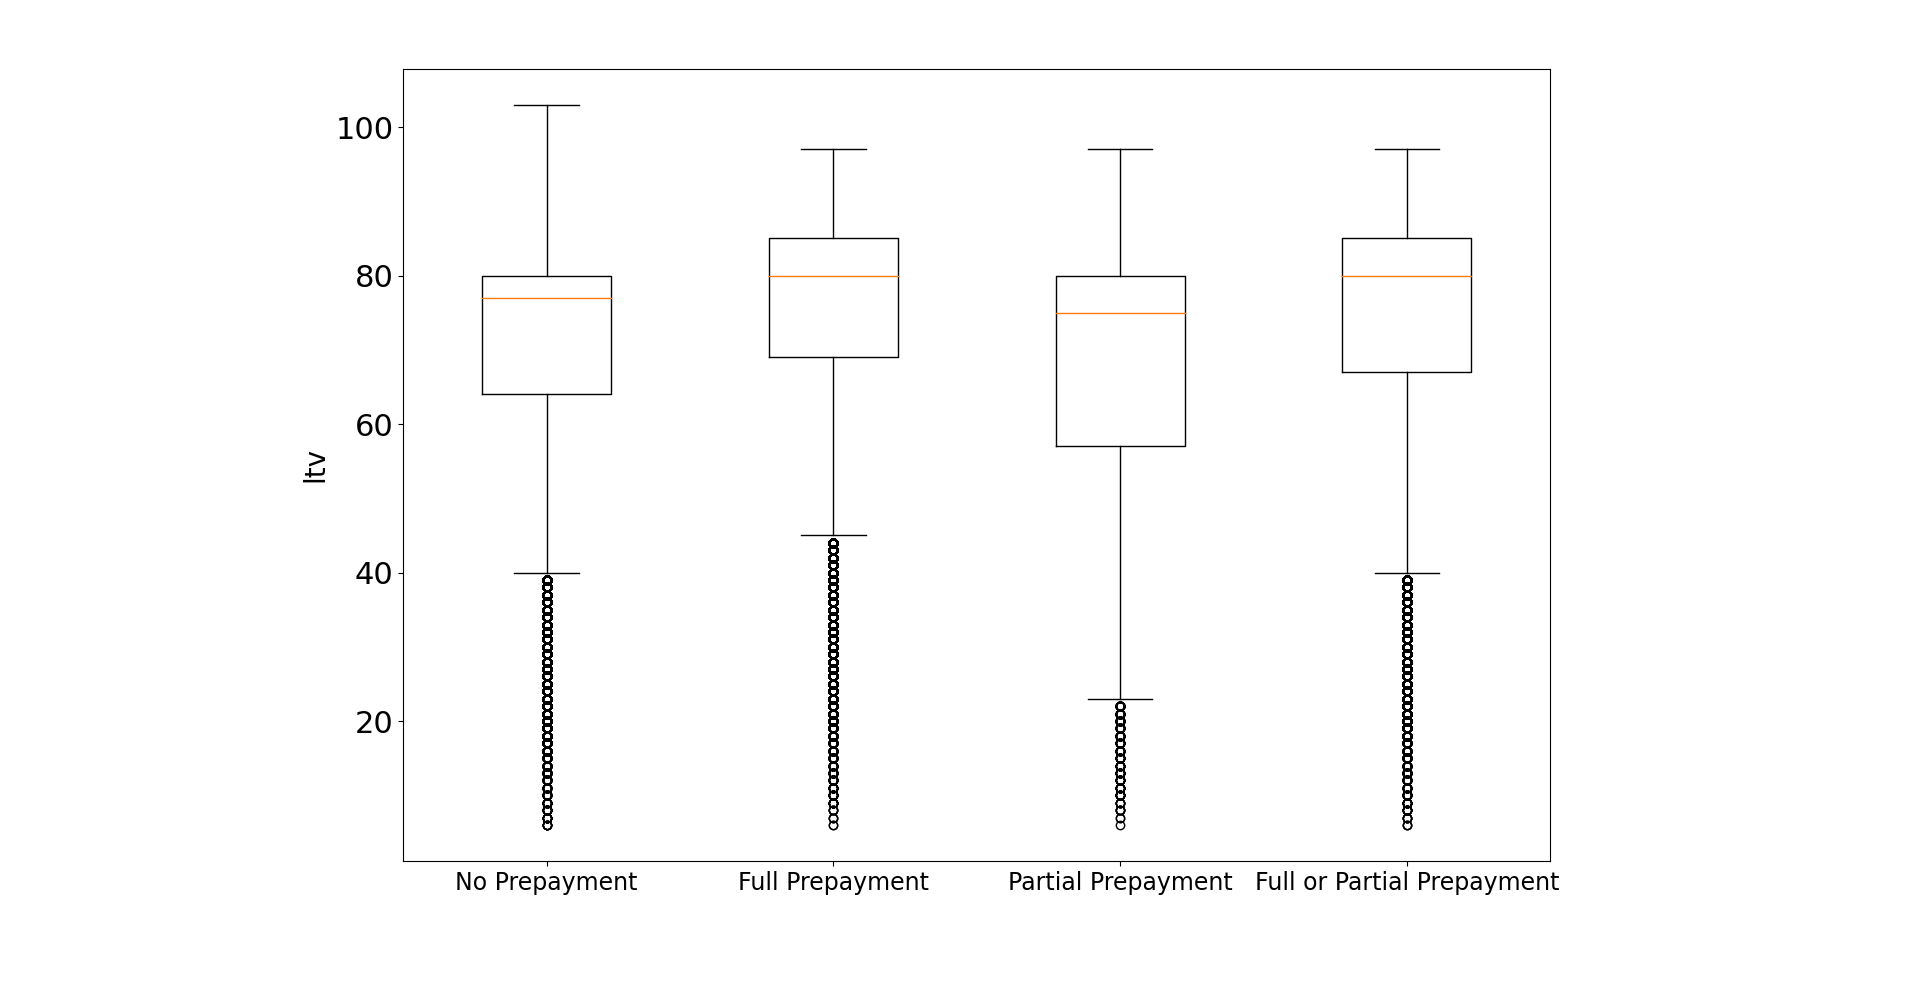
\includegraphics[width=\linewidth]{Latex/Report/Figures/Boxplot_of_ltv_[2013, 2014, 2015, 2016, 2017, 2018, 2019, 2020]_.png}
            \caption{
                Boxplot of LTV for sample data.
                 From left to right: No prepayment, 
                 Full prepayment, Partial prepayment and Full or 
                 Partial prepayment.
                 }
            \label{model_boxplot_LTV}
        \end{figure}
        Combining Figure \ref{model_boxplot_LTV} and Table 
        \ref{model_Pvals_of_LTV}, LTV can be considered as a 
        potential risk driver and needs further investigation. As 
        mentioned, one observes similar behaviour of the data through 
        the years. For further investigation, year 2013 is considered 
        as individual, as all years give similar results.  
        \\\\
        In Figure \ref{model_LTV_against_prepayment} the loans in 
        which no prepayments are made are filtered out of the data. 
        Higher magnitudes of LTV  observed, values around 80, which is 
        in accordance with Figure \ref{model_boxplot_LTV}. This figures 
        implies again that LTV could be a risk driver. 
        \begin{figure}[H]
            \centering
            \begin{subfigure}{0.45\textwidth}
                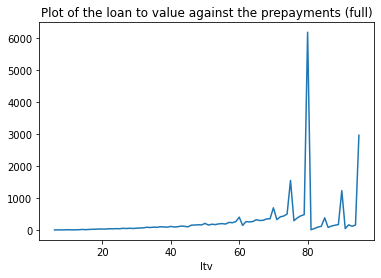
\includegraphics[width=\linewidth]{Latex/Report/Figures/LTV againts Full prepayments.png}
                \caption{
                    LTV against Full prepayments.
                    }
                \label{model_LTV_against_full_prepayment}
            \end{subfigure}
            \begin{subfigure}{0.45\textwidth}
                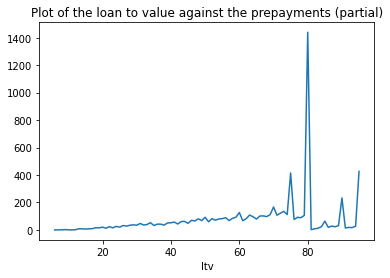
\includegraphics[width=\linewidth]{Latex/Report/Figures/LTV againts Partial prepayments.png}
                \caption{
                    LTV against Partial prepayments.
                    }
                \label{model_LTV_against_partial_prepayment}
            \end{subfigure}
            \caption{LTV against magnitude of prepayments.}
            \label{model_LTV_against_prepayment}
        \end{figure}
    
    \subsubsection{Original combined loan-to-value}
        As stated, both CLTV and LTV are calculated in similar ways. 
        To study the behaviour of CLTV in case of partial and full 
        prepayments, a boxplot is made. In Figure \ref{model_boxplot_CLTV} 
        one obverses a difference in behaviour. This behaviour is tested 
        using Kolmogorov Smirnov test as well, the obtained $p$-values 
        can be found in Table \ref{model_Pvals_of_CLTV}. All $p$-values 
        are zero which suggest independent data. A zero $p$-value could 
        however, correspond to too much data, as well.
        \begin{table}[H]
        \centering
            \begin{tabular}{lcl|c|c}
                \multicolumn{3}{c|}{Prepayment type} 
                & P-values& KS-statistic \\\hline
                No Prepayment & \& & Full Prepayment & 0 & 0.070947\\
                No Prepayment & \& & Partial Prepayment & 0 & 0.090918\\
                No Prepayment & \& & Full or Partial Prepayment & 0 & 0.053969 \\
                Full Prepayment & \& & Partial Prepayment & 0 & 0.150986
		    \end{tabular}
            \caption{
                $p$-values of CLTV (in which if both partial and full 
                prepayments happen, it is denoted as full prepayment).
                }
	        \label{model_Pvals_of_CLTV}
        \end{table}
        Further investigating year 2013 one observes similar behaviour 
        for CLTV, see Figure \ref{model_CLTV_against_prepayment}. 
        This behavior is similar as with LTV.
        \begin{figure}[H]
            \centering
            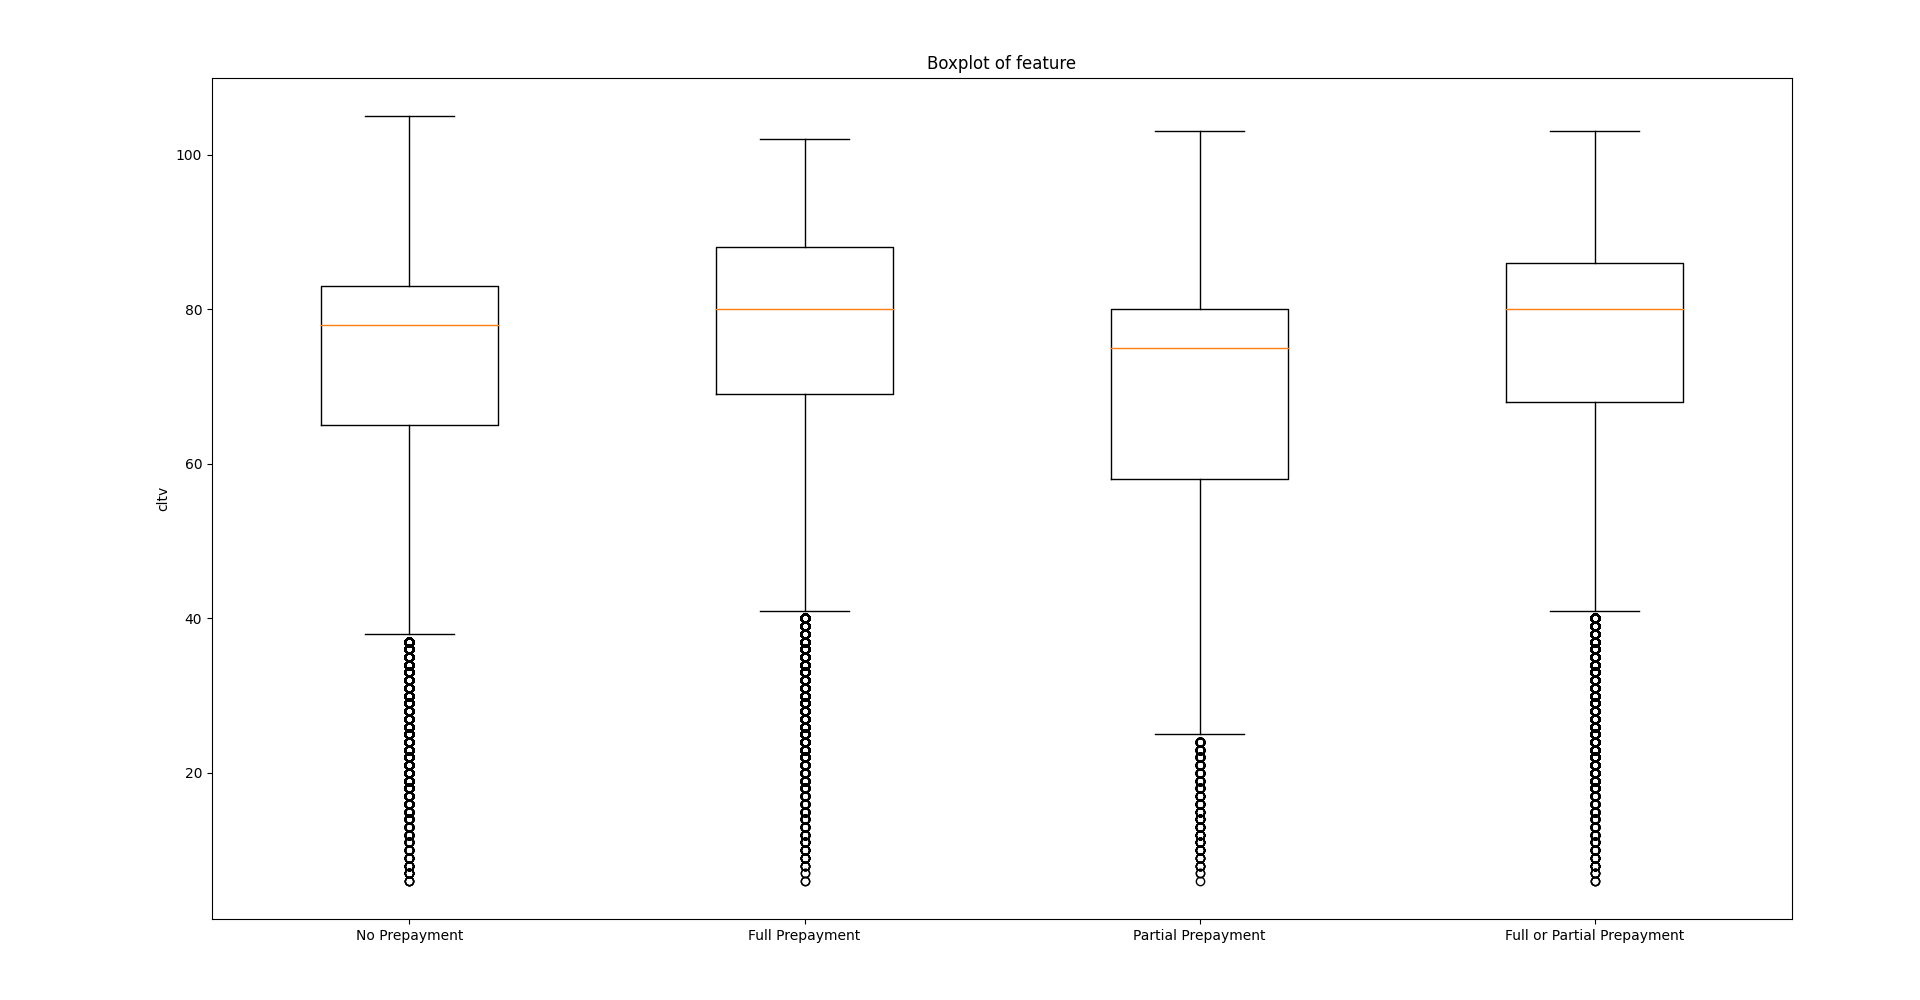
\includegraphics[width=\linewidth]{Latex/Report/Figures/Boxplot_of_cltv_[2013, 2014, 2015, 2016, 2017, 2018, 2019, 2020]_.png}
            \caption{
                Boxplot of CLTV of sample data. From left to right: 
                No prepayment, Full prepayment, Partial prepayment 
                and Full or Partial prepayment.
                }
            \label{model_boxplot_CLTV}
        \end{figure}
        \begin{figure}[H]
            \centering
            \begin{subfigure}{0.45\textwidth}
                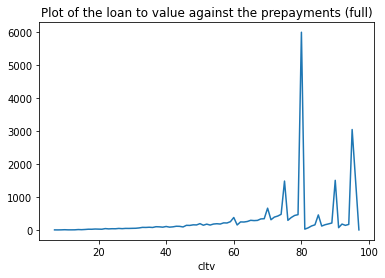
\includegraphics[width=\linewidth]{Latex/Report/Figures/CLTV againts Full prepayments.png}
                \caption{
                    CLTV against Full prepayments.
                    }
                \label{model_CLTV_against_full_prepayment}
            \end{subfigure}
            \begin{subfigure}{0.45\textwidth}
                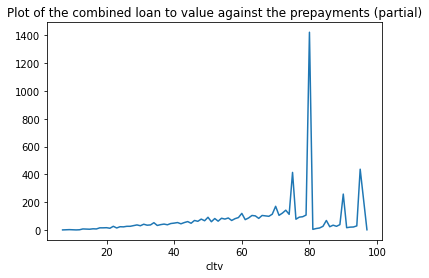
\includegraphics[width=\linewidth]{Latex/Report/Figures/CLTV againts Partial prepayments.png}
                \caption{
                    CLTV against Partial prepayments.
                    }
                \label{model_CLTV_against_partial_prepayment}
            \end{subfigure}
            \caption{
                CLTV against magnitude of prepayments.
                }
            \label{model_CLTV_against_prepayment}
        \end{figure}
        
    \subsubsection{Original unpaid principal balance}
        Another important characteristic of a loan is the UPB, 
        which denotes the value of the mortgage. This characteristic 
        is used to calculate both LTV and CLTV. From the 
        observations of CLTV and LTV it is expected that a loan 
        with high UPB with small purchase price is more likely 
        to be prepaid. However, a low UPB is also likely to be 
        prepaid as the money required to make a prepayment is 
        less in comparison to a high UPB. To see if this is in 
        accordance with the data a boxplot consisting all 
        sorts of prepayments is formed. In Figure 
        \ref{model_boxplot_UPB} one sees the UPB corresponding 
        to partial prepayments to be smaller than the UPB of no 
        prepayments. Which is in accordance with our last remark 
        about the behaviour of the UPB. On the other hand, the 
        UPB corresponding to full prepayments turns out to be 
        higher than the UPB of no prepayments. This is already 
        observed in the behaviour of LTV and CLTV. 
        \begin{figure}[H]
            \centering
            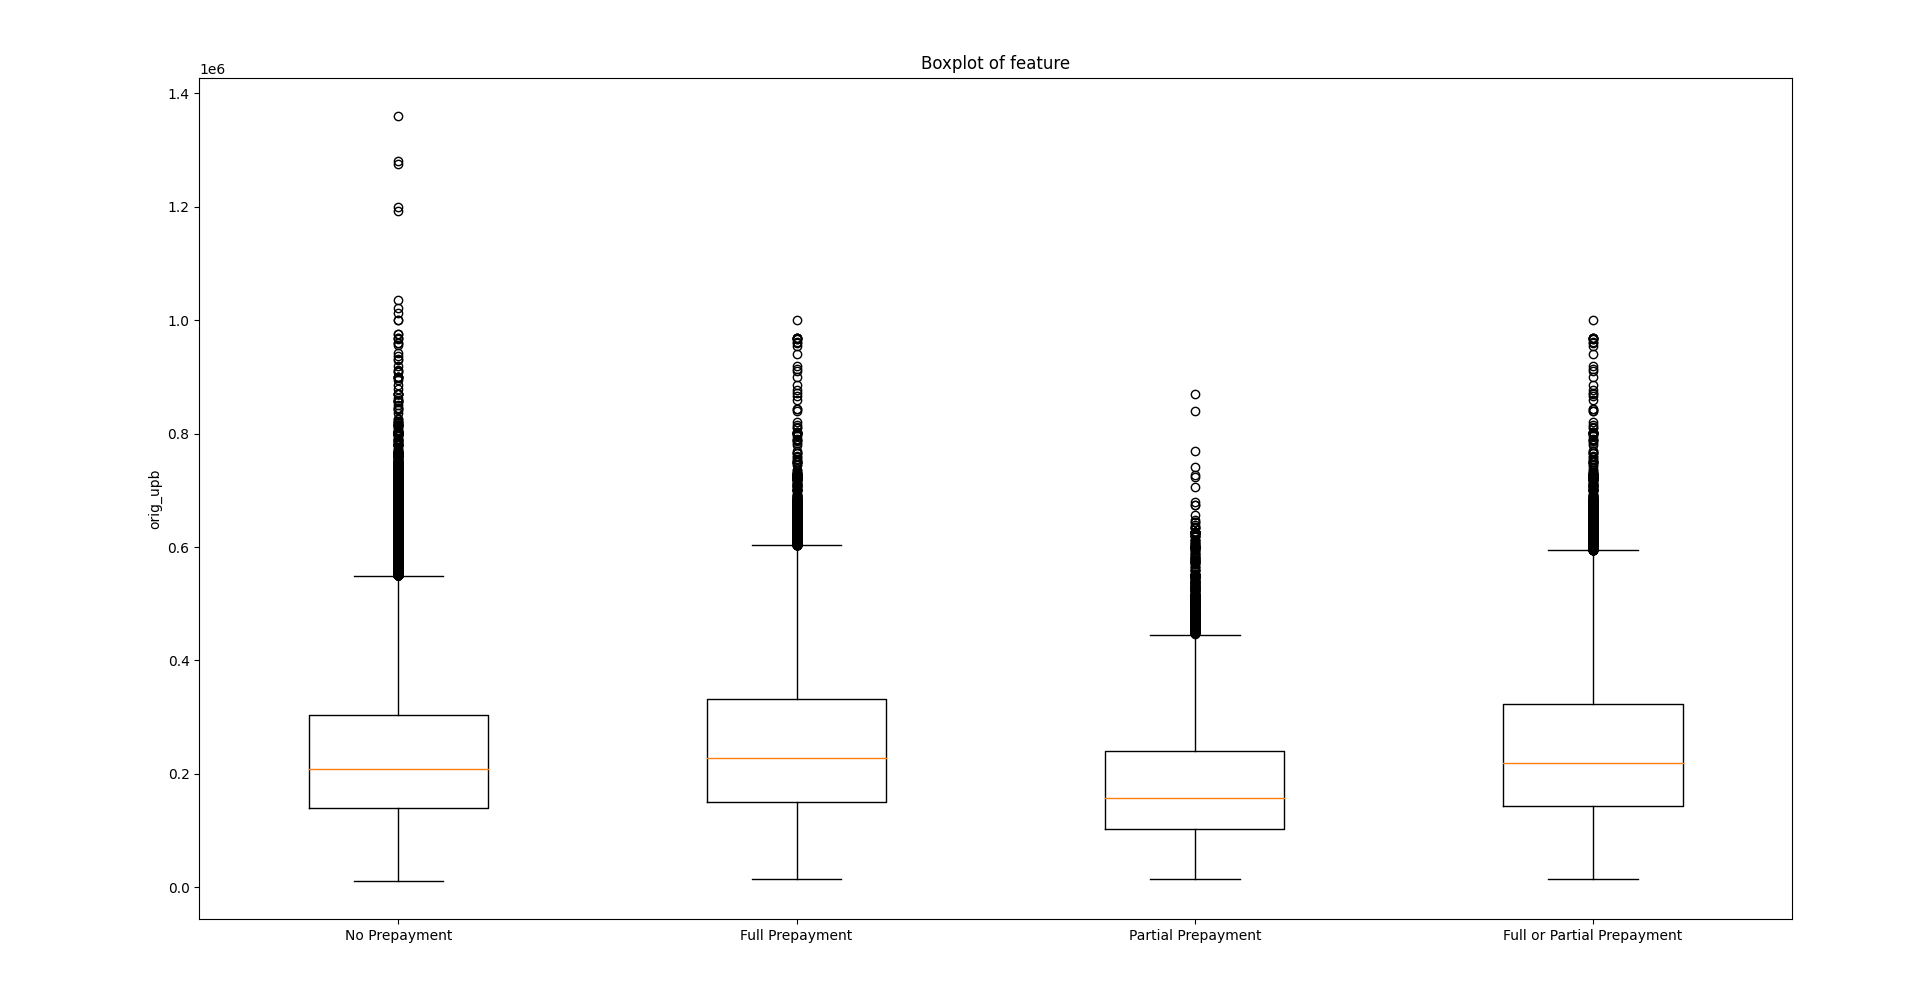
\includegraphics[width=\linewidth]{Latex/Report/Figures/Boxplot_of_upb_[2013, 2014, 2015, 2016, 2017, 2018, 2019, 2020]_.png}
            \caption{
                Boxplot of UPB for sample data. From left to right: 
                No prepayment, Full prepayment, Partial prepayment 
                and Full or Partial prepayment.
                }
            \label{model_boxplot_UPB}
        \end{figure}
        \noindent
        The dependence of the UPB is determined with use of 
        Kolmogorov Smirnov test, as well. In Table 
        \ref{model_Pvals_of_UPB}, all p-values are zero and hence 
        the data is independent. A zero p-value could however, also 
        correspond to too much data. 
        \begin{table}[H]
        \centering
            \begin{tabular}{lcl|c|c}
                \multicolumn{3}{c|}{Prepayment type} 
                & P-values& KS-statistic \\\hline
                No Prepayment & \& & Full Prepayment & 0 & 0.068385\\
                No Prepayment & \& & Partial Prepayment & 0 & 0.182088\\
                No Prepayment & \& & Full or Partial Prepayment & 0 & 0.043719 \\
                Full Prepayment & \& & Partial Prepayment & 0 & 0.238933
		    \end{tabular}
            \caption{
                $p$-values of UPB (in which if both partial and full 
                prepayments happen, it is denoted as full prepayment).
                }
	        \label{model_Pvals_of_UPB}
        \end{table}
        \noindent
        By isolation the data of year 2013, Figure 
        \ref{model_UPB_against_prepayment} is obtained. Here a smaller 
        UPB results in more prepayments. Hence, UPB is an 
        important characteristic to predict prepayments. 
        \begin{figure}[H]
            \centering
            \begin{subfigure}{0.45\textwidth}
                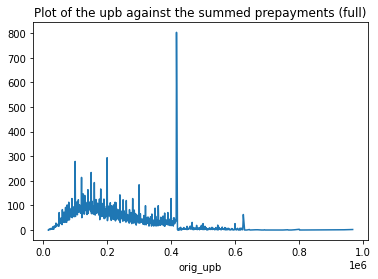
\includegraphics[width=\linewidth]{Latex/Report/Figures/UPB againts Full prepayments.png}
                \caption{
                    UPB against Full prepayments.
                    }
                \label{model_UPB_against_full_prepayment}
            \end{subfigure}
            \begin{subfigure}{0.45\textwidth}
                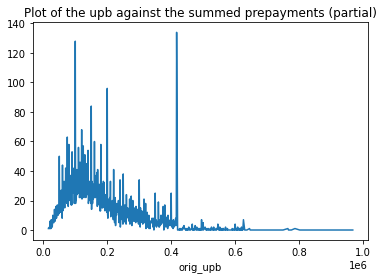
\includegraphics[width=\linewidth]{Latex/Report/Figures/UPB againts Partial prepayments.png}
                \caption{
                    UPB against Partial prepayments.
                    }
                \label{model_UPB_against_partial_prepayment}
            \end{subfigure}
            \caption{
                UPB against magnitude of prepayments.
                }
            \label{model_UPB_against_prepayment}
        \end{figure}
        
\subsubsection{Original interest rate}
    At last, the behaviour of characteristic original interest rate is 
    considered. It is expected that in loans with a higher interest 
    rate, more prepayments are made. This follows from getting a 
    loan somewhere else with lower interest rate and using this 
    money to prepay the original loan. The data is split based 
    on the kind of prepayment. This division is used to determine 
    possible dependence between this characteristic. The $p$-values 
    given in Table \ref{model_Pvals_of_int} suggest the data to 
    be independent. This test is performed on a large amount of 
    data and hence might be false. 
    \begin{table}[H]
        \centering
            \begin{tabular}{lcl|c|c}
                \multicolumn{3}{c|}{Prepayment type} & P-values& KS-statistic \\\hline
                No Prepayment & \& & Full Prepayment & 0 & 0.195919\\
                No Prepayment & \& & Partial Prepayment & 0 & 0.079967\\
                No Prepayment & \& & Full or Partial Prepayment & 0 & 0.165275 \\
                Full Prepayment & \& & Partial Prepayment & 0 & 0.263374
		    \end{tabular}
            \caption{
                $p$-values of interest rates (in which if both partial 
                and full prepayments happen, it is denoted as full 
                prepayment).
                }
	        \label{model_Pvals_of_int}
        \end{table}
    A boxplot comparing the prepayment might back up the $p$-values. 
    In Figure \ref{model_boxplot_int_rt}, a difference of behaviour 
    is seen based on the type of prepayment. A prepayment happens 
    more likely when the original interest rate is high. Which is 
    as expected. However, the partial prepayments turn out to be 
    made with smaller original interest rates. 
    \begin{figure}[H]
        \centering
        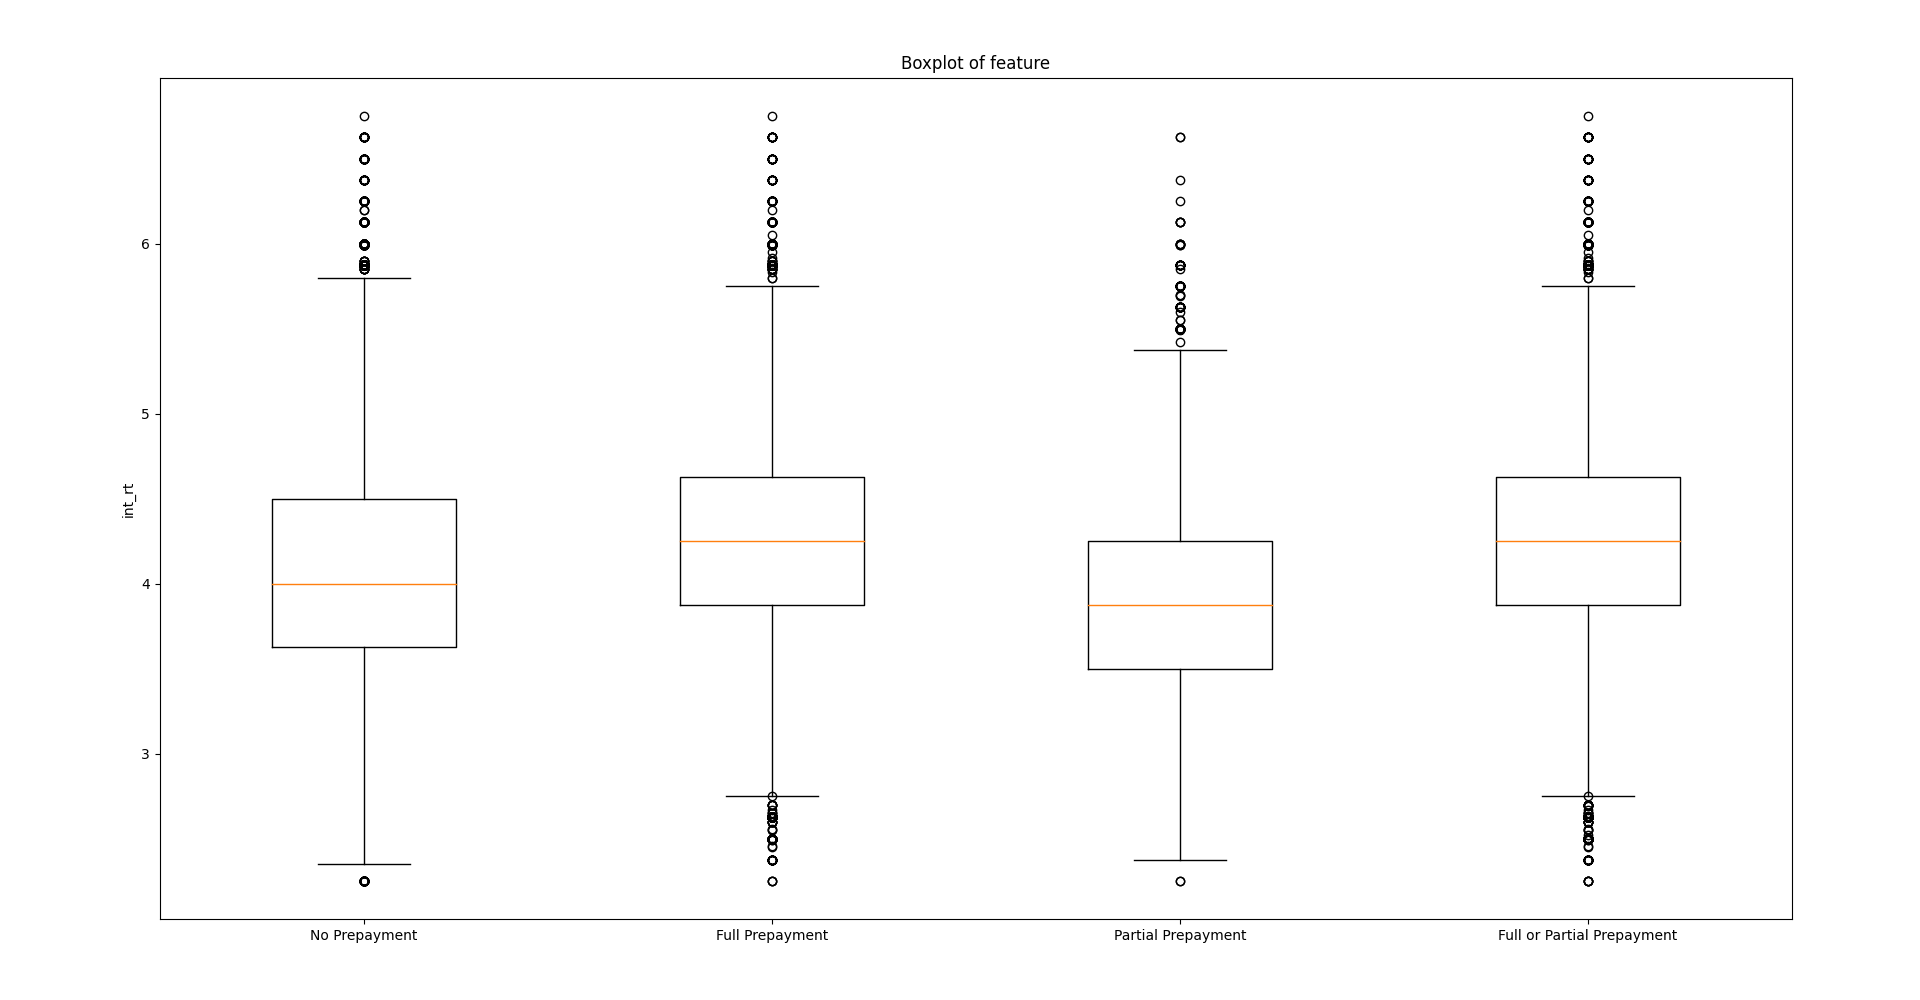
\includegraphics[width=\linewidth]{Latex/Report/Figures/Boxplot_of_int_rt_[2013, 2014, 2015, 2016, 2017, 2018, 2019, 2020]_.png}
        \caption{
            Boxplot of original interest rate of sample data. 
            From left to right: No prepayment, Full prepayment, 
            Partial prepayment and Full or Partial prepayment.
            }
        \label{model_boxplot_int_rt}
    \end{figure}
    \noindent
    The influence of the original interest rate of year 2013 can be 
    seen in Figure \ref{model_int_rt_against_prepayment}. Here, 
    one observes again a higher interest rate implying more 
    prepayments. Note the interest rate for full prepayments to 
    be higher than the interest rate of partial prepayments. 
    \begin{figure}[H]
        \centering
        \begin{subfigure}{0.45\textwidth}
            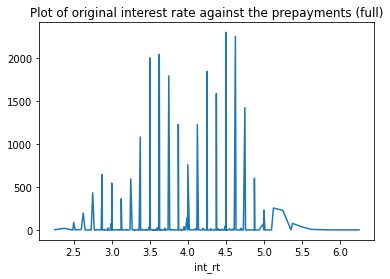
\includegraphics[width=\linewidth]{Latex/Report/Figures/int_rt againts Full prepayments.png}
            \caption{
                Interest rate against Full prepayments.
                }
            \label{model_int_rt_against_full_prepayment}
        \end{subfigure}
        \begin{subfigure}{0.45\textwidth}
            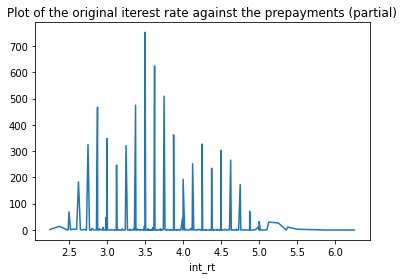
\includegraphics[width=\linewidth]{Latex/Report/Figures/int_rt againts Partial prepayments.png}
            \caption{
                Interest rate against Partial prepayments.
                }
            \label{model_int_rt_against_partial_prepayment}
        \end{subfigure}
        \caption{
            Original interest rate against magnitude of prepayments.
            }
        \label{model_int_rt_against_prepayment}
    \end{figure}
        
\subsection{Interest incentive}
    We can further investigate the interest rate as a risk factor. 
    Together with the originating and monthly payments files we 
    also have access to the Mortgage US 15 over all the weeks 
    between 2013 an 2020. This gives us the fixed interest rate 
    that US home-buyers would pay if they take out a loan lasting 
    15 years at a certain time.
    \begin{figure}[H]
        \centering
        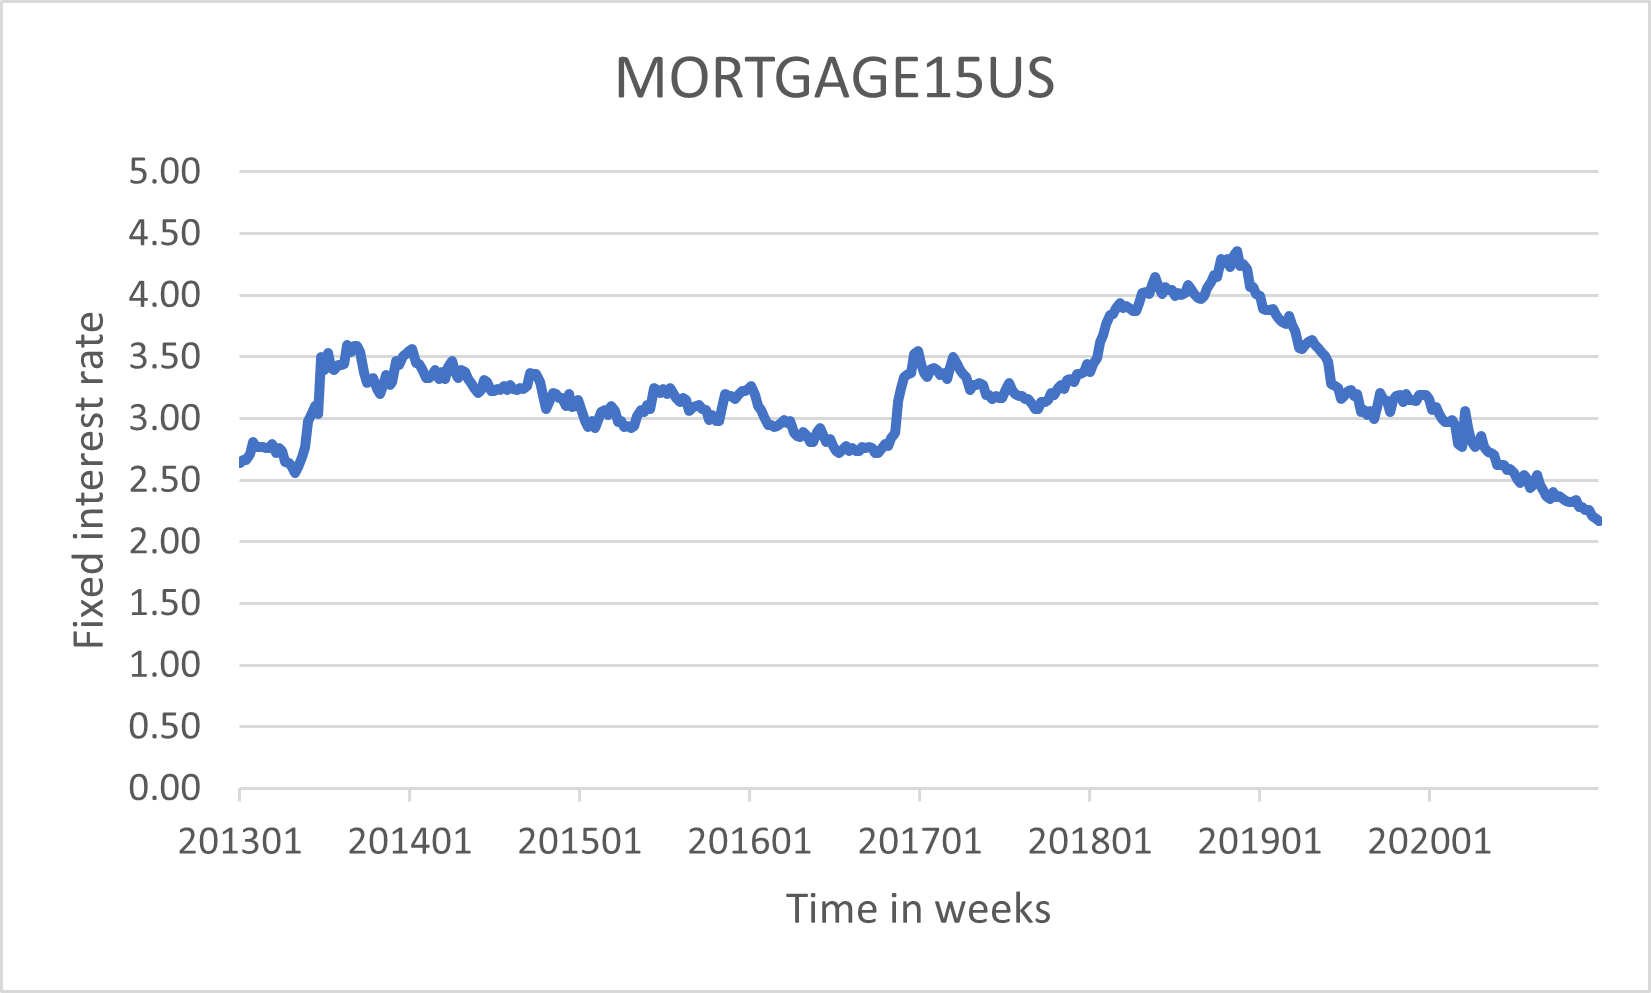
\includegraphics[scale=0.7]{Latex/Report/Figures/mortgage15US.png}
        \caption{
            Graph of fixed interest rate in US
            }
        \label{mortgage15us}
    \end{figure}
    The fixed interest rates for the beginning of a mortgage is 
    given to us per week. To determine the fixed interest rate 
    per month we take the maximum of the interest rates per week. 
    This values are also close to the fixed interest rates for 
    mortgages over 30 and 40 years, we can use this data to compare 
    with the loans of 30 and 40 years in our data set.
    \\\\
    We would expect when the interest rate of a loan is higher then 
    the fixed interest rate corresponding to that time, a loanee wants 
    to fully prepay his mortgage and take a new one for the lower 
    fixed interest rate. Of course the loanee must have the resources 
    to fully pay-off his loan. When the loanee does not have the 
    resources to fully prepay his mortgage, the loanee could make 
    a partial prepayment. To see this incentive as a risk factor we 
    first make a new variable: \textit{the interest incentive}. 
    The interest incentive is defined as the current interest rate 
    of the loan minus the fixed interest for that given time. 
    When the interest incentive is positive we expect that the loanee 
    might make a prepayment. To see how the interest incentive 
    is related to the prepayments we look at figure 
    \ref{pvals_incentive}. 
    \\\\
    The box plots shows that there is significant difference in 
    the behaviour of the interest incentive in months with no 
    prepayment compared to full prepayments. Besides, performing 
    a Kolmogorov Smirnov test and obtain the p-values as given 
    in Table \ref{pvals_incentive}. All p-values are zero implying 
    independent data. A zero p-value could however, also correspond 
    to too much data. 
    However, we do not see a clear difference between no 
    prepayments en the partial prepayments. So we assume that 
    the interest incentive only has effect on full prepayment 
    which sounds logical. If a loanee does not have enough 
    resources to fully prepay the loan, apparently it is not 
    interesting for them to do a partial prepayment. We will 
    now further investigate the relationship between the 
    interest rate incentive and the full prepayments.

    \begin{table}[H]
    \centering
        \begin{tabular}{lcl|c|c}
            \multicolumn{3}{c}{Prepayment type} & P-values& KS-statistic \\\hline
            No Prepayment & \& & Full Prepayment & 0 & 0.208387\\
            No Prepayment & \& & Partial Prepayment & 0 & 0.083474\\
            No Prepayment & \& & Full or Partial Prepayment & 0 & 0.0567477 \\
            Full Prepayment & \& & Partial Prepayment & 0 & 0.275293
	    \end{tabular}
        \caption{
            $p$-values of interest incentive.
            }
	    \label{pvals_incentive}
    \end{table}

    \begin{figure}[H]
        \centering
        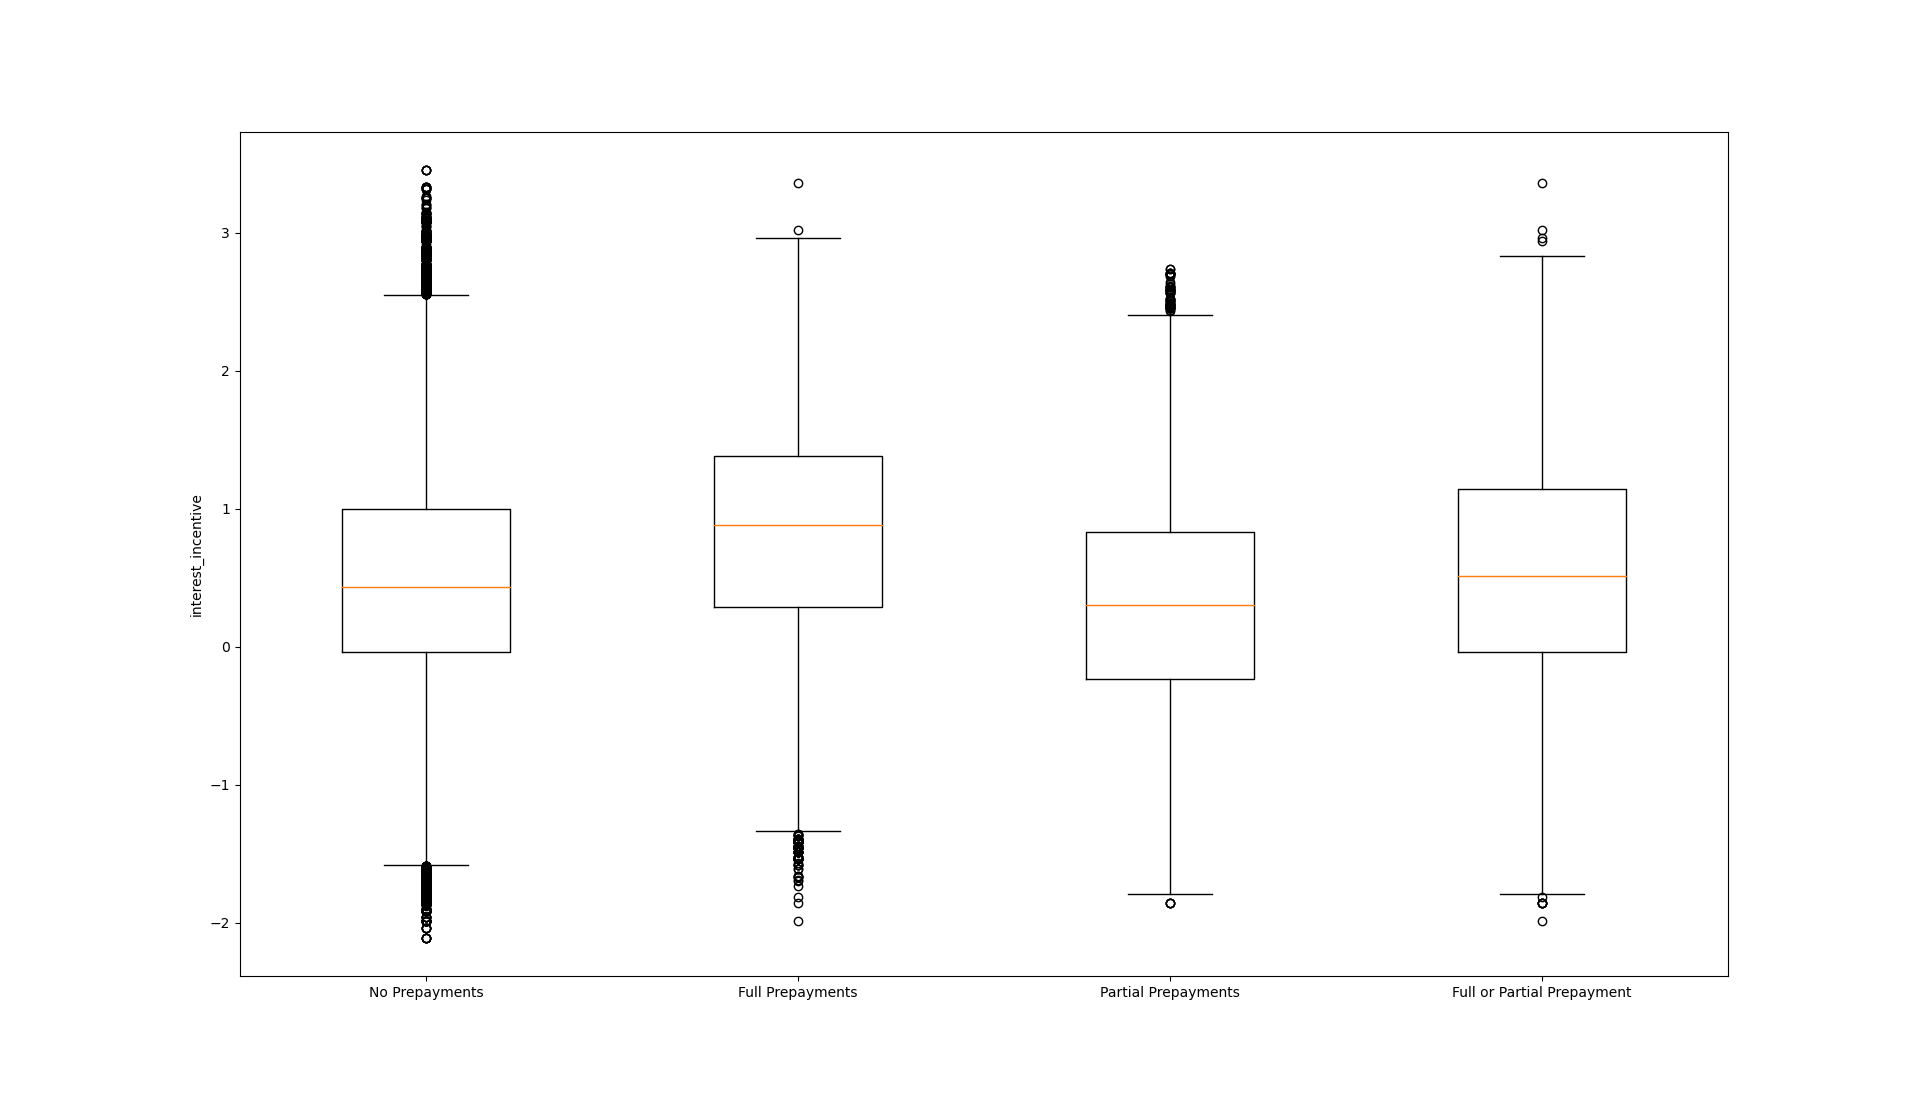
\includegraphics[width=\linewidth]{Latex/Report/Figures/Boxplots_interest_incentive.png}
        \caption{Boxplot of interest incentive for sample data. From left to right: No prepayment, Full prepayment, Partial prepayment and Full or Partial prepayment.}
        \label{boxplots_incentive}
    \end{figure}
        
To further investigate the relation between full prepayments and the interest incentive we want to take a look at the observed prepayment ratio. This is the ratio between the amount of debt which is full prepaid over all the loans and the total outstanding debt per month. This gives us a new variable which is unique per month. We can now take a look at the relation between this ratio and the interest incentive. We would expect that when the interest incentive goes up, this ratio will to. \\
We will visualize this relation with a scatter plot, where each dot will be bigger for the number of observations. Per different values of the ratio we will look at the corresponding interest rate incentives. The dot will then be placed on the mean of all these incentives. The size of the dot will be determined by the amount of interest incentive where this mean is based on. This results in a clear plot as seen in Figure \ref{scatter_interest}.

\begin{figure}[H]
            \centering
            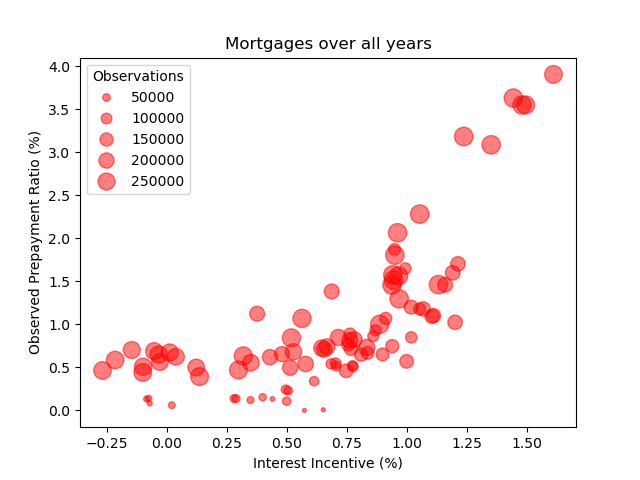
\includegraphics[scale=0.7]{Latex/Report/Figures/Bubbles_all_years.png}
            \caption{Scatter plot of the observed prepayment ratio against the incentive interest.}
            \label{scatter_interest}
        \end{figure}

From this we can conclude that the interest incentive does have a clear effect on the observed prepayment ratio. We do still see that with a negative interested incentive mortgage holders do still prepay. This can be because of all different reasons. The loanne could have had a equity injection or OTHER REASONS??!!